\documentclass[12pt]{article}
\usepackage{amsmath}
\usepackage{graphicx}
\usepackage{hyperref}
\usepackage[utf8]{inputenc}
\usepackage{listings}
\usepackage{xcolor}
\usepackage{graphicx}
\definecolor{codegreen}{rgb}{0,0.6,0}
\definecolor{codegray}{rgb}{0.5,0.5,0.5}
\definecolor{codepurple}{rgb}{0.58,0,0.82}
\definecolor{backcolour}{rgb}{0.95,0.95,0.92}

\lstdefinestyle{mystyle}{
    backgroundcolor=\color{backcolour},   
    commentstyle=\color{codegreen},
    keywordstyle=\color{magenta},
    numberstyle=\tiny\color{codegray},
    stringstyle=\color{codepurple},
    basicstyle=\ttfamily\footnotesize,
    breakatwhitespace=false,         
    breaklines=true,                 
    captionpos=b,                    
    keepspaces=true,                 
    numbers=left,                    
    numbersep=5pt,                  
    showspaces=false,                
    showstringspaces=false,
    showtabs=false,                  
    tabsize=2
}

\lstset{style=mystyle}


\title{Analisis Kompleksitas Algoritma Selection Sort Iterative dan Recursive}
\author{Analisis Kompleksitas Algoritma}
% \date{2021–01–05}
\begin{document}
\maketitle
\begin{center}
    
\includegraphics[width=8cm, height=8cm]{images/logo_telkom.png}
    \vspace{1cm}
    \\
    \textbf {Disusun oleh} \linebreak
    \\
    \begin{tabular}{ll}       
    Ni Made Dwipadini Puspitarini &(1301194141)\\
    Vena Erla Candrika &(1301194040)\\
    Claudia Mei Serin Sitio &(1301190424)\\
    Michael Putera Wardana &(1301194056)   
    \end{tabular}
\end{center}
\newpage
\section{Algoritma Selection Sort}
Selection sort adalah metode pengurutan yang melakukan pencarian elemen yang terbesar (jika diurutkan mengecil) dan terkecil (jika diurutkan membesar) kemudian melakukan pertukaran terhadap elemen tersebut ke bagian paling depan elemen - elemen yang belum terurut.
\subsection{Pseudo code}
\begin{figure}[h!]
    \centering
    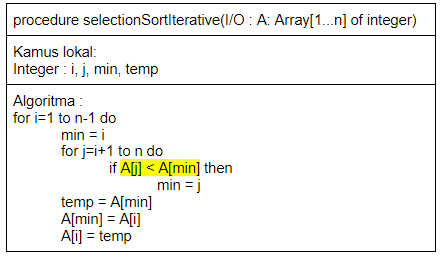
\includegraphics[width=1\textwidth]{images/pseudocodeIterative.PNG}
    \caption{psuedocode iterative selection sort}
\end{figure}
\newpage
\begin{figure}[h!]
    \centering
    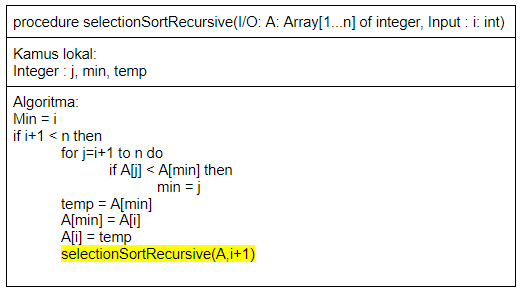
\includegraphics[width=1\textwidth]{images/pseudocodeRecursive.PNG}
    \caption{psuedocode recursive selection sort}
\end{figure}
\newpage
\subsection{Source code}
\begin{lstlisting}[language=Python]
# Procedure recursive selection sort
def selectionSortRecursive(A, i):
    min = i
    n = len(A)
    if i + 1 < n:
        for j in range(i + 1, n):
            if A[j] < A[min]:
                min = j
        temp = A[min]
        A[min] = A[i]
        A[i] = temp    
        selectionSortRecursive(A, i + 1)
\end{lstlisting}
\begin{lstlisting}[language=Python]
# Procedure iterative selection sort
def selectionSortIterative(A):
    for i in range(len(A) - 1):
        min = i
        for j in range(i + 1, len(A)):
            if A[j] < A[min]:
                min = j
        temp = A[min]
        A[min] = A[i]
        A[i] = temp
\end{lstlisting}
\newpage
\section{Worst Case dan Best Case}
Melakukan pengujian dengan menggunakan input size 100 yang sudah terurut membesar dan mengecil.
Data yang diujikan sebagai berikut :\\
$Best case = [0, 1, 2,\dotsc,98, 99]$\\
$Worst case = [100, 99, 98,\dotsc,2, 1]$\\
Dari hasil pengujian tersebut didapatkan hasil sebagai berikut :
\begin{verbatim}
=============================================
WORST CASE
Banyak data : 100
Iterative selection sort dieksekusi dalam 0.000434 detik
Recursive selection sort dieksekusi dalam 0.000436 detik
=============================================
BEST CASE
Banyak data : 100
Iterative selection sort dieksekusi dalam 0.000381 detik
Recursive selection sort dieksekusi dalam 0.000455 detik
=============================================
\end{verbatim}
Dari pengujian worst dan best case mendapatkan kesimpulan bahwa tidak ada worst dan best case tidak ada dalam algoritma selection sort
\newpage
\section{Pengujian}
Melakukan pengujian terhadap input size 10, 100, 500, 1000, dan 1500 acak.\\
Data yang diujikan sebagai berikut :\\
$10 = [480, 699, 1172,\dotsc,210, 1511]$\\
$100 = [991, 403, 298, 169,\dotsc,41, 178, 984]$\\
$500 = [156, 2, 1043, 308, 1415,\dotsc, 891, 526, 99]$\\
$1000 = [397, 1507, 727, 466,\dotsc, 504, 1417, 1613]$\\
$1500 = [719, 471, 319, 510,\dotsc,  193, 593, 819]$\\
Dari hasil pengujian tersebut didapatkan hasil sebagai berikut :
\begin{verbatim}
=========================
Banyak data : 10
Iterative selection sort dieksekusi dalam 0.000020 detik
Recursive selection sort dieksekusi dalam 0.000019 detik
=========================
Banyak data : 100
Iterative selection sort dieksekusi dalam 0.000337 detik
Recursive selection sort dieksekusi dalam 0.000385 detik
=========================
Banyak data : 500
Iterative selection sort dieksekusi dalam 0.008802 detik
Recursive selection sort dieksekusi dalam 0.009498 detik
=========================
Banyak data : 1000
Iterative selection sort dieksekusi dalam 0.040314 detik
Recursive selection sort dieksekusi dalam 0.039260 detik
\end{verbatim}

\newpage

\begin{verbatim}
=========================
Banyak data : 1500
Iterative selection sort dieksekusi dalam 0.084786 detik
Recursive selection sort dieksekusi dalam 0.089137 detik
=========================
\end{verbatim}

\newpage
\section{Analisis Kompleksitas}
\subsection{Basic operation}
\begin{figure}[h!]
    \centering
    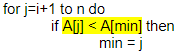
\includegraphics[width=0.5\textwidth]{images/iterative.PNG}
    \caption{basic operation iterative selection sort}
\end{figure}
\begin{figure}[h!]
    \centering
    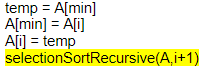
\includegraphics[width=0.5\textwidth]{images/recursive.PNG}
    \caption{basic operation recursive selection sort}
\end{figure}
\subsection{Perhitungan kompleksitas waktu}
\subsubsection{Iterative}
\begin{align}
    C(n) &=\sum_{i=1}^{n-1} \sum_{j=i+1}^{n} 1 = \sum_{i=1}^{n-1} {n-(i+1)+1} =\sum_{i=1}^{n-1} {n-i}
    \nonumber
    \\
    &= n\sum_{i=1}^{n-1} 1 - \sum_{i=1}^{n-1} i = n\sum_{i=1}^{n-1} 1 - \frac{(n-1)n}{2}
    \nonumber
    \\
    &= n(n-1) - \frac{(n-1)n}{2}
    \nonumber
    \\
    &= \frac{(n-1)n}{2} \approx \frac{1}{2}n^2 \in O(n^2)
\end{align}
\subsubsection{Recursive}
\begin{align}
    M(n) =
    \begin{cases}
        0 & \quad n \leq 1\\
        M(n-1) + n - 1  & \quad n > 1
    \end{cases}
\end{align}
    
\begin{align}
    M(n) &=M(n-1) + n -1
    \nonumber
    \\
    &= (M(n-2) + n -1) + n - 1
    \nonumber
    \\
    &= M(n-2) + 2n - 2
    \nonumber
    \\
    &= (M(n-3) + n-1) + 2n - 2
    \nonumber
    \\
    &= M(n-3) + 3n - 3
    \nonumber
    \\ \vdots
    \nonumber
    \\
    &= M(n-i) + in-i
    \nonumber
    \\
    n-i &= 1, \text{ sehingga } i = n - 1
\end{align}

\begin{align}
    \text{maka, }M(n-i) + in - i &= M(n-(n-1)) + (n-1)n - (n-1)
    \nonumber
    \\
    &= M(n-n+1) + n^2 - n - n + 1
    \nonumber
    \\
    &= M(1) + n^2 - 2n+1
    \nonumber
    \\
    &= 0 + n^2 - 2n + 1
    \nonumber
    \\
    &= n^2 - 2n + 1 \in O(n^2)
\end{align}
\subsection{Notasi Asimtotik}
Algoritma selection sort memiliki notasi asimtotik yang sama baik iterative maupun recursive yaitu $O(n^2)$
\subsection{Class Efficiency}
Algoritma selection sort memiliki class efficiency yaitu \textbf{Quadratic}
\newpage
\section{Analisis Tambahan}
Dari hasil pengujian didapatkan data sebagai berikut :
\begin{table}[h!]
    \centering
    \begin{tabular}{|l|l|l|}
    \hline
    N   & Iterative (s) & Recursive (s) \\ \hline
    10	&0.000020	&0.000019\\ \hline
100	&0.000337	&0.000385\\ \hline
500	&0.008802	&0.009498\\ \hline
1000	&0.040314	&0.039260\\ \hline
1500	&0.084786	&0.089137\\ \hline    
    \end{tabular}
    \caption{hasil pengujian execution time}
\end{table}
\begin{figure}[ht!]
    \centering
    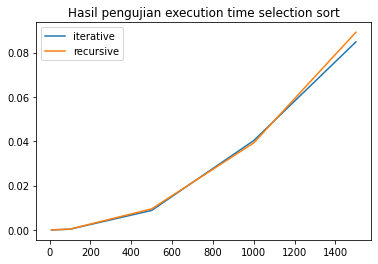
\includegraphics[width=0.8\textwidth]{images/output_27_1.png}
    \caption{line plot hasil pengujian execution time}
\end{figure}
\begin{figure}[ht!]
    \centering
    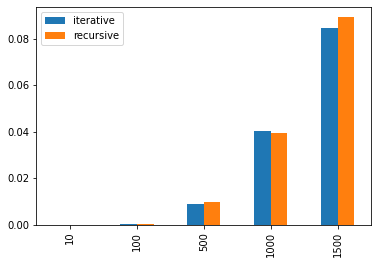
\includegraphics[width=0.8\textwidth]{images/output_28_1.png}
    \caption{bar plot hasil pengujian execution time}
\end{figure}
\newpage
\section{Kesimpulan}
Dapat disimpulkan bahwa :
\begin{enumerate}
    \item Tidak memiliki best case dan worst case
    \item Kompleksitas algoritma selection sort adalah $O(n^2)$
\end{enumerate}
\section{Sumber dan Referensi}
\begin{enumerate}
    \item \href{https://www.techiedelight.com/selection-sort-iterative-recursive/}{Algoritma Selection Sort}
    \item \href{https://github.com/krobus00/Tubes-AKA}{Repository github Tubes-AKA}
    \item \href{https://colab.research.google.com/drive/1NBGprozO0wrKurCJ-q1EM0LyCBFzYKkK?usp=sharing}{Google Colaboratory Tubes-AKA}
\end{enumerate}
\end{document}